\subsection{Convex Hamiltonians}
\label{subsec:preliminaries-convex-hamiltonian-language}

The smooth characteristic line field has a convex-analytic formulation that
continues to make sense when \(\partial K\) is not smooth.  For a convex body
\(K\) containing the origin, its support and gauge functions are
\[
  h_K(y)\coloneqq\max_{x\in K}\langle x,y\rangle,
  \qquad
  g_K(x)\coloneqq\inf\{r>0:x\in rK\}.
\]
The boundary is the level set \(g_K=1\).  We use the convex,
\(2\)-homogeneous Hamiltonian
\[
  H_K(x)\coloneqq g_K(x)^2.
\]
For a convex function \(H\), its subdifferential at \(x\) is
\[
  \partial H(x)
  =\{y:H(z)\geq H(x)+\langle y,z-x\rangle
    \text{ for every }z\}.
\]
When \(H\) is differentiable, this set consists only of \(\nabla H(x)\).

\begin{definition}[Contact-normalized generalized characteristic]
\label{def:preliminaries-generalized-characteristic}
A \emph{contact-normalized generalized characteristic} on \(\partial K\) is
a curve \(\gamma\in W^{1,2}([0,T],\mathbb R^4)\), with \(T>0\) and
\(\gamma(0)=\gamma(T)\), whose image lies in \(\partial K\) and which satisfies
\begin{equation}\label{eq:preliminaries-generalized-characteristic}
  -J_0\dot\gamma(t)\in\partial H_K(\gamma(t))
  \quad\text{for almost every }t\in[0,T].
\end{equation}
\end{definition}

For smooth \(K\), the subdifferential in
\eqref{eq:preliminaries-generalized-characteristic} is the singleton
\(\{\nabla H_K\}\).  The resulting Hamiltonian vector is tangent to the
characteristic line on \(\partial K\).  Thus the definition recovers the Reeb
orbits described above, including their parametrization.
\begin{figure}[htbp]
  \centering
  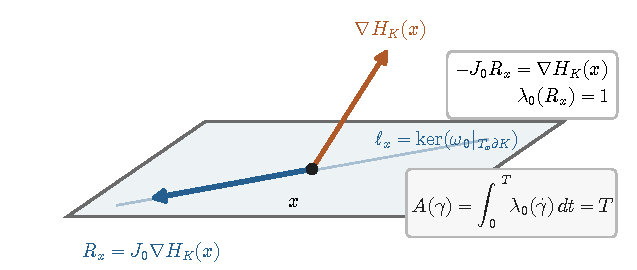
\includegraphics[width=0.94\linewidth]
    {figures/foundations/characteristic-normalization.pdf}
  \caption{The characteristic and contact normalizations at a smooth boundary
  point.  This is a dimension-reduced tangent-space schematic: it records that
  \(R_x=J_0\nabla H_K(x)\) spans the characteristic line inside
  \(T_x\partial K\), but projected angles and lengths carry no meaning.  The
  contact condition \(\lambda_0(R_x)=1\) turns elapsed time into action.}
  \label{fig:preliminaries-characteristic-normalization}
\end{figure}

The normalization also persists without smoothness.  Indeed, if
\(y\in\partial H_K(x)\), then the \(2\)-homogeneity of \(H_K\) gives
\[
  \langle y,x\rangle=2H_K(x).
\]
Along a generalized characteristic, \(H_K(\gamma)=1\), and hence
\[
  \lambda_0|_{\gamma(t)}(\dot\gamma(t))
  =\frac12\langle-J_0\dot\gamma(t),\gamma(t)\rangle
  =1
  \quad\text{for almost every }t.
\]
Consequently every contact-normalized generalized characteristic satisfies
\begin{equation}\label{eq:preliminaries-generalized-characteristic-action-period}
  A(\gamma)=T.
\end{equation}

This formulation separates the general nonsmooth dynamical object from its
finite description on a polytope.  The latter will follow by calculating the
subdifferential of \(H_K\) from the active facets.
